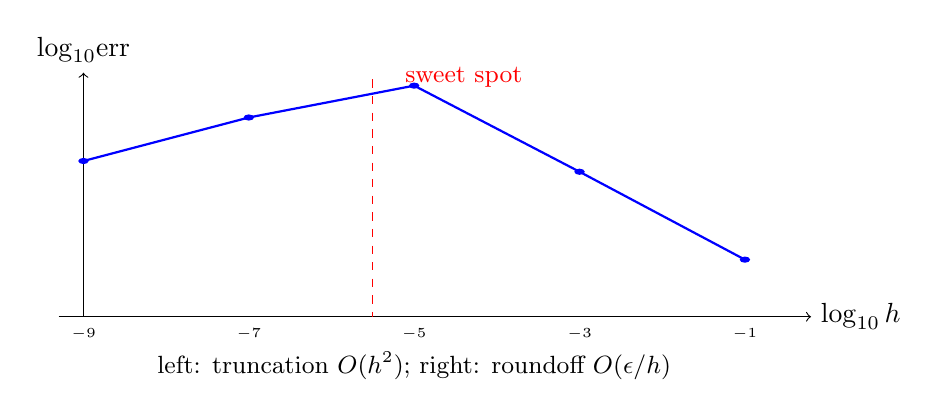
\begin{tikzpicture}[xscale=1.05,yscale=0.62]
\draw[->] (-9.3,0)--(-0.2,0) node[right]{$\log_{10}h$};
\draw[->] (-9,0)--(-9,5) node[above]{$\log_{10}$err};
% data: h=1e-1:2.486e-3->-2.6; 1e-3:2.486e-7->-6.6; 1e-5:3.0e-11->-10.5; 1e-7:8.5e-10->-9.07; 1e-9:8.2e-8->-7.09
% y = (-log10 err)*0.45 so lower err = higher point
\foreach \x/\e in {-1/2.60,-3/6.60,-5/10.52,-7/9.07,-9/7.09}{
  \fill[blue] (\x,{0.45*\e}) circle (1.8pt);}
\draw[blue,thick] (-1,{0.45*2.60})--(-3,{0.45*6.60})--(-5,{0.45*10.52})--(-7,{0.45*9.07})--(-9,{0.45*7.09});
\draw[dashed,red] (-5.5,{0.45*10.8})--(-5.5,0);
\node[red] at (-4.4,4.9) {\small sweet spot};
\node at (-5,-1.0) {\small left: truncation $O(h^2)$; right: roundoff $O(\epsilon/h)$};
\foreach \x/\l in {-1/{\(-1\)},-3/{\(-3\)},-5/{\(-5\)},-7/{\(-7\)},-9/{\(-9\)}}{\node at (\x,-0.35) {\tiny \l};}
\end{tikzpicture}
